\section{Создание графического интерфейса с помощью библиотеки swing}
\subsection{Обработка событий}


\begin{frame}[fragile]
	\frametitle{Обработка событий}

	\large{}
	\begin{enumerate}
	\item{Понять, какое событие вы хотите обработать (примеры: когда выделяют элемент списка, когда подводят курсор мыши к кнопке, когда нажимают клавишу на клавиатуре)}
	\item{Постараться придумать название для такого события (List, Mouse, Key)}
	\item{В описании класса компонента нати все функции вида \emph{add<...>Listener} (addListSelectionListener, addMouseListener, addKeyListener)}
	\item{Обычно один "Listener" служит для обработки нескольких видов событий, например addKeyListener добавляет обработчик и нажатия и отпускания клавиши. В качестве параметров в эти методы передается класс, реализующий соостветствующий интерфейс (ListSelectionListener, MouseListener, KeyListener)}
	\end{enumerate}
\end{frame}

\begin{frame}[fragile]
	\frametitle{Обработка событий}

	\begin{enumerate}
	\setcounter{enumi}{5}
	\item{Посмотреть документацию по интерфейсу и найти среди методов подходящий (например mouseEntered - курсор подводят к компоненту)}
	\item{Реализовать интерфейс в своем классе, который будет обрабатывать события (описать там все методы из интерфейса и добавить implements MouseListener в заголовок класса)}
	\item{Добавить свой обработчик (обычно это делают там где создается компонент, надо вызвать метод addMouseListener)}
	\item{Обычно в методы-обработчики событий передается объект-событие, который содержит дополнительную информацию, например MouseEvent содержит координаты курсора и нажатые кнопки}
	\end{enumerate}

\end{frame}

\subsection{Layouts}

\begin{frame}[fragile]
	\frametitle{Layouts}
	\begin{minted}[bgcolor=bgcode,linenos=true]{java}
	JFrame frame = new JFrame();
	JPanel panel = frame.getContentPane();

	BoxLayout l;
	l = new BoxLayout(panel, BoxLayout.Y_AXIS);
	panel.setLayout(l);

	b = new JButton("Button 1");
	panel.add(b);

	b = new JButton("B 2");
	panel.add(b);
	\end{minted}
\end{frame}

\begin{frame}[fragile]
	\frametitle{BoxLayout}
	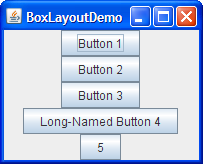
\includegraphics[scale=1]{BoxLayoutDemo.png}
\end{frame}

\begin{frame}[fragile]
	\frametitle{BorderLayout}
	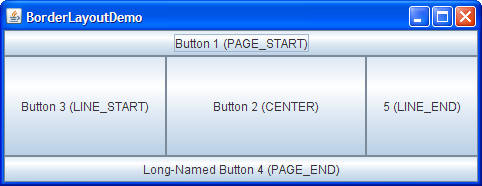
\includegraphics[scale=0.7]{BorderLayoutDemo.png}
\end{frame}

\begin{frame}[fragile]
	\frametitle{GridBagLayout}
	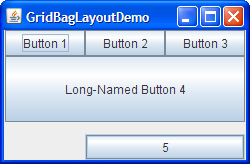
\includegraphics[scale=1]{GridBagLayoutDemo.png}
\end{frame}

\begin{frame}[fragile]
	\frametitle{GridLayout}
	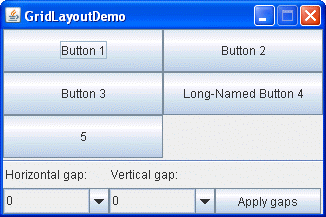
\includegraphics[scale=1]{GridLayoutDemo.png}
\end{frame}

\begin{frame}[fragile]
	\frametitle{FlowLayout}
	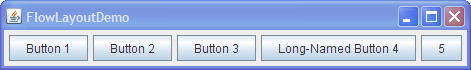
\includegraphics[scale=0.8]{FlowLayoutDemo.png}
\end{frame}

\begin{frame}[fragile]
	\frametitle{GroupLayout}
	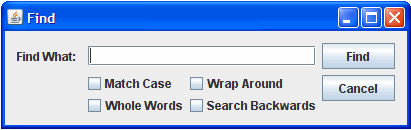
\includegraphics[scale=1]{find.png}
\end{frame}

\begin{frame}[fragile]
	\frametitle{SpringLayout}
	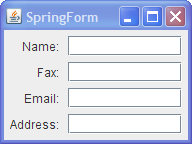
\includegraphics[scale=1]{SpringForm.png}
\end{frame}


